\chapter{Methods}
\label{chap:methods}
\section{Overview}
Here is a breakdown of the workflow from MD to charge transport in the order of the workflow as we used it in
this work. 
MorphCT is developed to facilitate charge characterization of morphological data. It takes GSD files which are
the native file format of the simulation engine HOOMD-blue \cite{Anderson2020a}. The morphologies used to
obtain the data for this work were obtained from equilibrium Molecular Dynamics simulations. 
All the tools used to implement, analyze, and
visualize this work are freely available. 

\section{Molecular Dynamics}

    \subsection{MD Computational Methods}
Here we introduce the software stack for plankton and also introduce singularity and docker whcih we can call
back to when we say morphCT has a FLOW but it needs work in improvements.
The ITIC morphology was simulated using Plankton-Flow (https://github.com/cmelab/planckton-flow) on Fry, the high performance computing cluster at Boise State University. Planckton-Flow is a dataspace manager that uses
singularity, docker and signac to contanerize a package developed to facilitate simulating self-assembly in
organic photovoltaic materials; Planckton (https://github.com/cmelab/planckton).

\section{Chromophores}

The term ``chromophore'' arose in a biochemical context and is generally defined
as a light-absorbing group or molecule \cite{biochemistry}.
In this context, a chromophore is often associated with the color of a material.
This is because, mechanistically, a photon collides with a chromophore, the absorbed energy
excites an electron from the highest occupied molecular orbital (HOMO) to the
lowest unoccupied molecular orbital (LUMO). As the chromophore relaxes to its
ground state, it releases a photon with wave length $\lambda = \frac{\hbar c}{E}$,
where $\hbar$ is Plank's constant, $c$ is the speed of light, and $E$ represents the
energy difference of the HOMO and LUMO. 

For the materials of interest to our research, it would be undesirable for a chomophore to relax to its ground
state and release a photon as this would consistute a loss mechanism. In the case of
OPVs we want our molecules bear that photo-electric
excitation long enough to jump to a nearby chromophore, and proceed, through a
series of quantum tunneling events, towards an electrode. 
In our work, a chromophore is defined as a region over which the
LUMO(HOMO for acceptor) of an excited molecular segment is thought to fully delocalized, creating a free
charge carrier. It is under this assumption that we execute a hopping model of charge transfer between
chromophores.  

    \subsection{Chromopore software}

A place to mention grits and VMD for chromophore delineation. Having made a choice about where chromoohores
are locatied in the morph we then need to build a neighborlist. 

\section{Chromophore Neighbors}

\begin{figure}
  \center
%\includegraphics[width=25cm]{figures/crystalline_voronoi.png}
  \includegraphics[width=0.8\linewidth]{figures/crystalline_voronoi_smaller.png} 
 % \includegraphics[width=\linewidth]{figures/crystalline_voronoi_smaller.png}
  \caption{2D Voronoi}
  \label{fig:2d}
\end{figure}


Again, with 15000 choose 2 pairs, we are required to perform some neighborlisting prior to QCC. so categorize chromophores as
neihgbors if they share an edge in the voronoi cells around the geometric center of the chromphore. Here, the
cell edges are drawn in a Euclidean way, with lines representing the set of points equidistant from a point
and its geometrically closest neighbor across the line. This analysis takes place in three dimensions. As a
demonstration a voronoi analysis was run on a 2D analogue of the crystalline P3HT system described elsewhere.
In figure [FIGURE], 15,000 thousand dots represent the single-monomer chromophore's geometric centers projected
in the xy-plane.Here,
a voronoi cell for any given chromophore center is the set of points that are closer to that chromophore
center than any other chromophore center. We use voronoi because BLAH. Euclidean space searching algorithms of
this sort are known to scale with $O(n\log{n})$ in the worst case and as low as $O(n)$ in the average case
\cite{Bentley1980}.
However as can seen from the figure, two points can share cell edges despite being rather far apart. We
therefore, further remove pairs from the neighborlist if they are far enough apart such that it is justifyable
to assume they do not interact electronically enough to effect to charge mobility calculation. This parameter will
depend on the material under investigation as was as the size of the individual chromophores. We tested the
sensitivity of the algorithm to the value (dcut). The figure shows the effect of cutoff distance on value of
calculated mobility. There is a diminishing return on computation around dcut 10. 


    \subsection{Voronoi software}

Utilizing the freud.locality.Voronoi() 
With a neighbor list built, a single charges movement through the morphology can be simulatied with the
application of a KMC algorthym.

\section{Marcus and QCC}

    \subsection{QCC software}

\section{Kinetic Monte Carlo}

Taking a charge carrier to be a quasi-particle inserted into a MD generated morpholgy, a KMC
simulation can be run on the bases of Marcus theory and quantum chemical analysis.

With each chromophore taken to be a discrete object, both in python, and with respect to its frontier
molecular orbitals, a charge hopping (transfering) from an excited chromophore to a neighboring chromophore can be modeled
as a discrete event that occurs at a rate. In our case the rate is estimable by semiclassical Marcus elctron transfer theory. With that,
the rate that a charge
will hop from chromophore $i$ to chromophore $j$, $k_{ij}$, is given by the
following equation:

\begin{align}
    k_{ij}  =  |T_{ij}|^2\ \frac{2\pi}{\hbar \sqrt{4 \pi \lambda_{ij} k_{B} T}}\ \exp{\Bigg[ \frac{(\Delta
    E_{ij} - \lambda_{ij})^2}{ 4 \pi \lambda_{ij} k_{B} T} \Bigg] }
\end{align}

with Botzmann's consant, $k_{B}$, and Planck's constant, $\hbar$. The parameters $T_{ij}$, $\lambda_{ij}$,
$\Delta E_{ij}$, $T$ represent th electronic overlap, the reorganization energy, the free energy difference, and
temperature. These are discussed in further detail in the results section, wherin we test the senseitivity of
the KMC results to these parameters individually. 
The accuracy of the marcus rate is thus dependent on the accuracy with which the inputs can be estimated. In
the following section we outline our quantum chemical treatment of both $T_{ij}$ and $\Delta E_{ij}$.

Taking $k_{ij}$ to be and
accurate rate of the electron transfer reaction, we implant a charge randomly into the morphology, calculate
the rate of all possible hops(events)
and put them in order of quickest to slowest to form a queue. The hop rate, $k_{ij}$, from the occupied chromophore to any
given neighbering chromophore is taken to be
inversely proportional to the amount of time, $\tau$, that the system will have to wait before that hop will
take place. However, hopping processes at the angstrom level do not proceed deterministically. 
Our implementation, and others like it [NEED REFS?], have
successfully captured the stochasticiity of these systems via a shuffling hopping queue.
The wait time for every potential hop from occupied chromophore $i$ onto a
neighboring chromophore $j$ looks as follows:

\begin{align}
    \tau = \frac{1}{k_{ij}} \cdot \ln{\frac{1}{x}} 
\end{align}
where x is a random number between 0 and 1 and $\log{(1/x)}$ is a scaling factor. To illucidate this
graphically, $\ln{(1/x)}$ is plotted in figure \ref{fig:ln} from 0 to 1. From this we can see that with
a large enough sampling, significant reshuffling of the queue will take place, allowing for a rare hop to jump
the queue.

\begin{figure}
  \center
  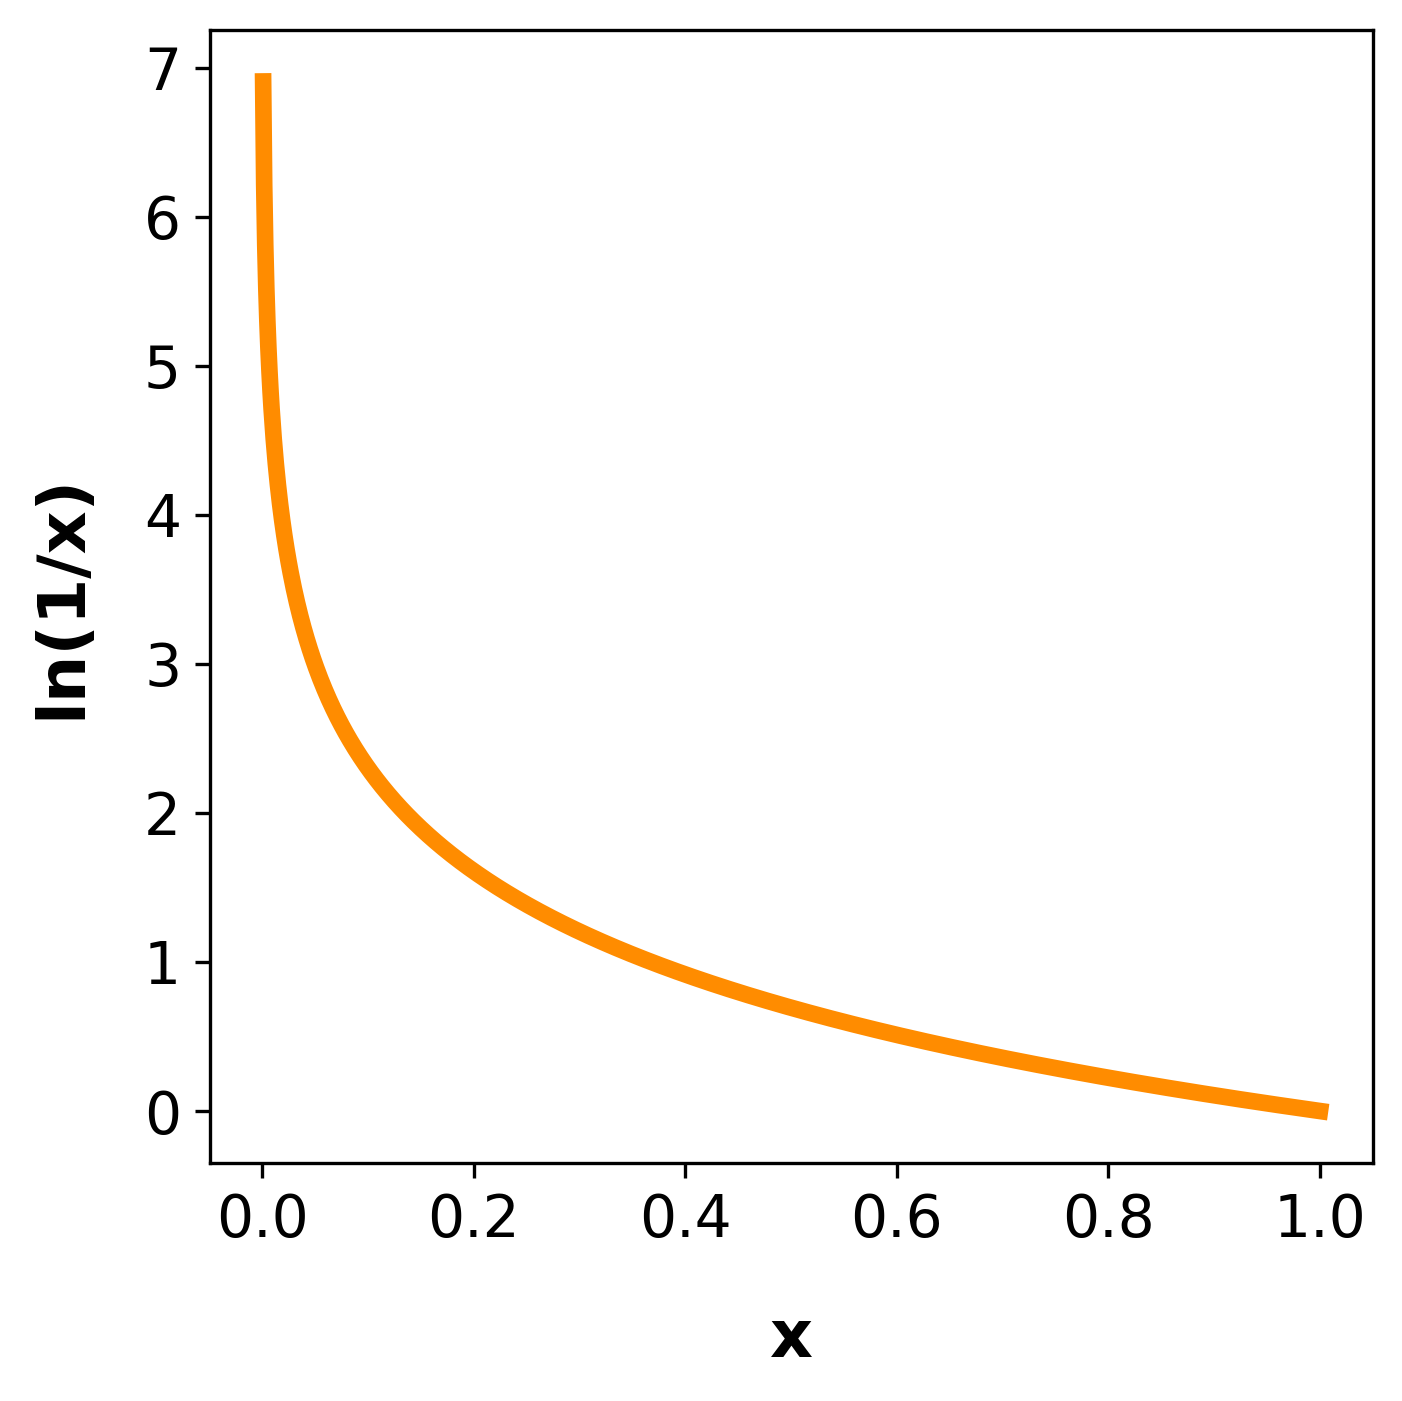
\includegraphics[width=0.8\linewidth]{figures/naturallog.png}
  \caption{Graphical insight into the reshuffling of the wait time queue. Here the x-axis represents the 
    interval from which numbers are drawn randomly such that the wait times in the queue can be scaled 
    by ln(1/x).}
  \label{fig:ln}
\end{figure}

From the rationally shuffled queue, the shortest waittime (quickest available hop) is chosen and the charge is moved to
its new chromophore host. The system is then considered to have moved forward in time by $\tau$. This proceeds
until the charge carrier stalls out or hops past a prespecified lifetime. 


    \subsection{KMC software aka MorphCT}

\section{KMC analysis}

n overview of the KMC algorithm is given followed by a discription of the salient computational tools and
methods used to implement and optimize this implemention. 


\subsection{MSD Analysis}

The choice of carrier lifetimes effectively serve as checkpoints at which the displacement of charge carriers is recorded. For
each specified lifetime, a prescribed number individual KMC simulations is run as described above. When a
given charge carrier hops past the specified lifetime, that is, the addition of the current iterations $\tau$ advances
the simulation beyond the specified lifetime,  its displacement from its starting location is stored in the carrier object. After repeating this over a
statistically significant number of carriers, the carrier data can be aggregated and the mean squared
displacement(MSD) for a particle in the system and that lifetime can be estimated.
It is known that the MSD of a diffusive particle increases linearly as time goes to infinity. 
The slope of the MSD, $D$,  as time
goes to inifinity can be estimated as a linear fit between the MSD's at the specified lifetimes.

There is no objective best practice for determing the slope of the MSD as
time goes to inifinty from simulation data of this kind \cite{Maginn2018}. With that, we seek primarily to simplifiy the MSD analysis as much as
possible so as to accuratley report this stage of the analysis for clarity but also to facilitate apples to
apples comparisons to future works using this workflow. 

Finally, the results of the MSD analysis are then used to determine the zero-field mobility using the following Einstein-Smoluchowski relation:

\begin{align}
    \mu_{0} = \frac{eD}{6k_{B}T},
\end{align}

where $e$ is the elemental charge of a charge carrier, $D$ is the diffusion coefficient, $k_{B}$ is Planck's
constant and $T$ is temperature.  

A benifit to Monte Carlo analysis of this type is that charge carriers can be simultaneously. It is considered
to be "embarrasingly parrel," in that the subprocesses(charge carriers) require no communication.
MorphCT utilizes the python multiprocessing module to divide the prescribed number of charge carriers to be
simulated accross all available cores.  

\section{Quantum Chemical Methods}
At the core of Morphct is the estimation of HOMO (for donor) and LUMO (acceptor). This is because 
the inputs into the Marcus hopping equation are the offsets between neighboring  chromophores energy levels
determine the driving force and the TI is estimated using a dimer method that also uses the homo level. 
With that said, quantum chemical methods give us a framework from which to estimate the homo/lumos. A litany of
methods that use approximations and parameterizations to transform cumbersome ab initio quantum mechanical 
calculations into efficient algorithms for determining the electronic structure of a given compound. Morpcht 
leverages MINDO/3, a variation of the INDO(Intermediate Neglect of Differential Overlap) method,
which is an approximation method that seeks recreate the ab initio Hartree-Fock
results, where the Hatree-Fock theory allows for an iteratively convergent numerical solution to the Shrodinger equation.\cite{Thiel2014}. Calculating electronic structure with this method has
shown good agreement with experimental data and more rigorous Quantum chemical
methods 
\cite{Bredas2002}. Furthermore, variations in TI do not effect mobility calcs
that much (one of evans papers said this).  Results
from the this work compare well to jones2017 which implemented ZINDO/s, another
semi-empirical method. The
previous version of MorphCT utilized ORCA to provide the quantum chemical
approximations required to implement
a hopping model of charge transport \cite{Neese2012b}. Jones2017 showed that with this you can connect MD
provided morphology to charge transport characteristics. A particular 
choice of method comes down to how well we can organize a workflow and integrate the QQC portion of the
workflow modularly. This is because the quantum computational chemistry is a nascent and evolving field of its
own, with quickly increasing efficiencies and accuracies. Therefor, an important consideration is, "how can we
deintigrate and reintigrate a QCC software, tests its efficiency and accuracy, and do it in a way that lays
the groundwork to upgrade or swap it as better options emerge?". 

The software chosen to implement this method is
provided by pySCF (Python-based Simulations of Chemistry Framework) \cite{Sun2018a}. This framework
was chosen in the interest of reproducability and extensibility. PySCF is implemented almost entirly in the Python 
language, which is becoming increasingly ubiquitous in the scientific computing community. Furthermore,
ORCA's proprietary licensing was prohibitive in the efforts to containerize MorphCT for use on cluster and for
creating reproducible results. 
Solving shrodingers equation across tens of thousands of 
chromophores, which will be required to model an OPV material on the order of 10 nm, is untenable. Therefore
justified but drastic simplifications are necessary. Computation of the eigenvalues of the HOMO and HOMO-1
molecular orbitals of the dimer Hamiltonian requires the computation of three integrals: 
the site energy integral, the transfer integral (electronic overlap), and the overlap integral (physical
overlap). Neglecting the latter using an implementation of an INDO method can provide an effective transfer
integral. It is this approximation that allows an estimating of the transfer integral from the calculation of
the dimer splitting energy and the site energy. A further approximation, which is more relevant for highly regular chromopheres is Koopman's
approximation, which further neglects the site energy integral, thereby assuming all chromophores have the same
energetics in isolation.  \cite{Huang2005b}. Other studies have implemented DFT at this stage of predicting
mobility from molecular arrangement to good effect \cite{Deng2004}. The P3HT morphologies discussed in the evaluation section of the results
consist of 1000 oligomers of 15 repeating molecular units. Assigning each molecular unit as a chromophore
gives 15000 indivual QQC calculations and as many as 15000 choose 2 Dimer QCC calculations. The latter is
drastically lower because not all chromophores interact. In this workflow neighbor, finding is accomplished via
voronoi analysis. Nevertheless, with the volume of calculations necessary to simulate materials into the
nanometer range, DFT is prohibitively slow. 

 Implementing a hopping simulation requires the delineation of
individual segments of delocalization or chromophores. For polymeric materials like P3HT, MorphCT
can identify chromophores with a provided SMILES string. For less regular molecules, explicitly delineating
which atoms belong to which chromophores is required. At this stage of the workflow, consideration needs to be
given to where a charge may delocalize within. With ITIC, the frontier molecular orbitals, that is, the HOMO
and LUMO have negligible electron density along the side chains. With that, significant computational resources
can be conserved by leaving these atoms out of the of the QCC stage. To test this on ITIC we delineate the
backbone and the whole molecule and compare carrier mobility NEED THIS DATA. 



%%% Local Variables: 
%%% mode: latex
%%% TeX-master: "BSUmain"
%%% End: 
